% -----------------------------------------------------------------------------
% The MIT License (MIT)
%
% Copyright (c) 2015 Pejman Ghorbanzade
%
% Permission is hereby granted, free of charge, to any person obtaining a copy
% of this software and associated documentation files (the "Software"), to deal
% in the Software without restriction, including without limitation the rights
% to use, copy, modify, merge, publish, distribute, sublicense, and/or sell
% copies of the Software, and to permit persons to whom the Software is
% furnished to do so, subject to the following conditions:
%
% The above copyright notice and this permission notice shall be included in
% all copies or substantial portions of the Software.
%
% THE SOFTWARE IS PROVIDED "AS IS", WITHOUT WARRANTY OF ANY KIND, EXPRESS OR
% IMPLIED, INCLUDING BUT NOT LIMITED TO THE WARRANTIES OF MERCHANTABILITY,
% FITNESS FOR A PARTICULAR PURPOSE AND NONINFRINGEMENT. IN NO EVENT SHALL THE
% AUTHORS OR COPYRIGHT HOLDERS BE LIABLE FOR ANY CLAIM, DAMAGES OR OTHER
% LIABILITY, WHETHER IN AN ACTION OF CONTRACT, TORT OR OTHERWISE, ARISING FROM,
% OUT OF OR IN CONNECTION WITH THE SOFTWARE OR THE USE OR OTHER DEALINGS IN
% THE SOFTWARE.
% -----------------------------------------------------------------------------

\section*{Question 1}
Write a program \texttt{ShapeDiamond.java} that asks for an integer number \texttt{n} and using \texttt{*} characters, prints a diamond in \texttt{2n-1} rows, such that there is one \texttt{*} character in first row, three \texttt{*} characters in second row and $2n-1$ characters in $n$th row.
Figure \ref{fig1} shows a sample diamond created when user has entered 4 as input integer.
\begin{verbbox}
   *
  ***
 *****
*******
 *****
  ***
   *
\end{verbbox}
\begin{figure}[H]\centering
\theverbbox
\caption{Sample diamond generated in 7 rows} \label{fig1}
\end{figure}

\section*{Question 2}
Remember the Dalton Brothers? Neglecting their original heights, write a program \texttt{Daltons2.java} that asks for heights of Joe, William, Jack and Averell, as well as the order in which they have to be sorted in terms of height. The order is either \texttt{ASC} for shortest to tallest or \texttt{DESC} for tallest to shortest. The program should give names of the brothers in order of their heights as specified.
\newpage

\section*{Question 3}

\begin{wrapfigure}{r}{0.5\textwidth}
\centering
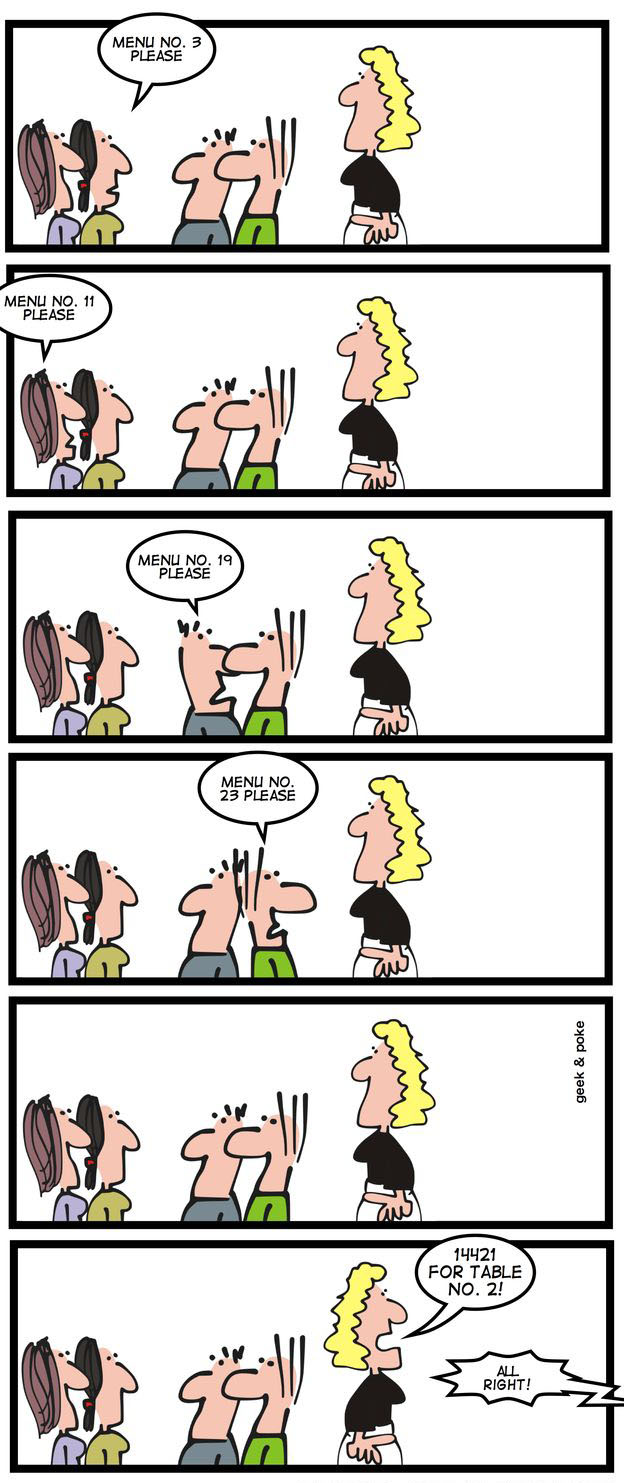
\includegraphics[width=0.5\textwidth]{\topDirectory/template/images/primeMenu.jpg}
\end{wrapfigure}

Minnie and Mannie are students of mathematics. Their area of interest is prime numbers. They also work part time in a restaurant. To fight the extreme boredom of their routine tasks at work, they have invented a little somewhat challenging game between themselves.

Minnie, the waitress, has numbered each item in the menu with a unique \textbf{random} prime number. When Minnie takes orders of a table, she will multiply the menu numbers of all orders placed by that table and gives the final multiplication to Mannie, the chef.

Thanks to his brilliant mind, Mannie will in less than two seconds decompose the given number to its prime factors and prepares the menu numbers corresponding to those factors.

Unfortunately, Mannie is absent this week and you have to replace him. As it is likely that you cannot decompose a number as fast as Mannie, you are requested to write a program \texttt{PrimeMenu.java} that asks for an integer number and prints all prime factors that number is divisible by. Obviously, your program should also indicate how many times the number is divisible by each prime number.
\newpage
